%%%%%%%%%%%%%%%%%%%%%%%%%%%%%%%%%%%%%%%%%
% Memo
% LaTeX Template
% Version 1.0 (30/12/13)
%
% This template has been downloaded from:
% http://www.LaTeXTemplates.com
%
% Original author:
% Rob Oakes (http://www.oak-tree.us) with modifications by:
% Vel (vel@latextemplates.com)
%
% License:
% CC BY-NC-SA 3.0 (http://creativecommons.org/licenses/by-nc-sa/3.0/)
%
%%%%%%%%%%%%%%%%%%%%%%%%%%%%%%%%%%%%%%%%%

\documentclass[letterpaper,11pt]{texMemo} % Set the paper size (letterpaper, a4paper, etc) and font size (10pt, 11pt or 12pt)

\usepackage{parskip} % Adds spacing between paragraphs
\usepackage{algorithm}
\usepackage[noend]{algpseudocode}
\usepackage{listings}
\usepackage{xcolor}
\usepackage{float}
\usepackage{hyperref}

\algdef{SE}[DOWHILE]{Do}{doWhile}{\algorithmicdo}[1]{\algorithmicwhile\ #1}

\setlength{\parindent}{15pt} % Indent paragraphs

%----------------------------------------------------------------------------------------
%	MEMO INFORMATION
%----------------------------------------------------------------------------------------

\memoto{Professor O'Connell} % Recipient(s)

\memofrom{Michael Brodskiy} % Sender(s)

\memosubject{CP3H} % Memo subject

\memodate{Monday, \today} % Date, set to \today for automatically printing todays date

\memoattach{7 (3 Figures, 2 Pseudocode, 2 Source code)}

\logo{\includegraphics[width=0.3\textwidth]{logo.png}} % Institution logo at the top right of the memo, comment out this line for no logo

%----------------------------------------------------------------------------------------

\begin{document}

\maketitle % Print the memo header information

%----------------------------------------------------------------------------------------
%	MEMO CONTENT
%----------------------------------------------------------------------------------------

\section*{Introduction}

The purpose of this document is to analyze the transient response curves and maximum weld times for certain mixes of tin/lead in thermocouples, generated by a combination of MATLAB and C++ scripts.

\section*{Steady-State Cooling}

\subsection*{Thermocouple Response}

As shown in \ref{fig:1}, the transient response curve is \underline{not} linear. Logically, this makes sense as the rate at which an object cools down is proportional to the difference between the object and its surrounding environment, as made evident through Newton's Law of Cooling. In this manner, as the thermocouple weld cools down, the rate at which it cools down is decreasing (\textit{i}.\textit{e}.\ the function is concave downwards).

\begin{figure}[H]
  \centering
  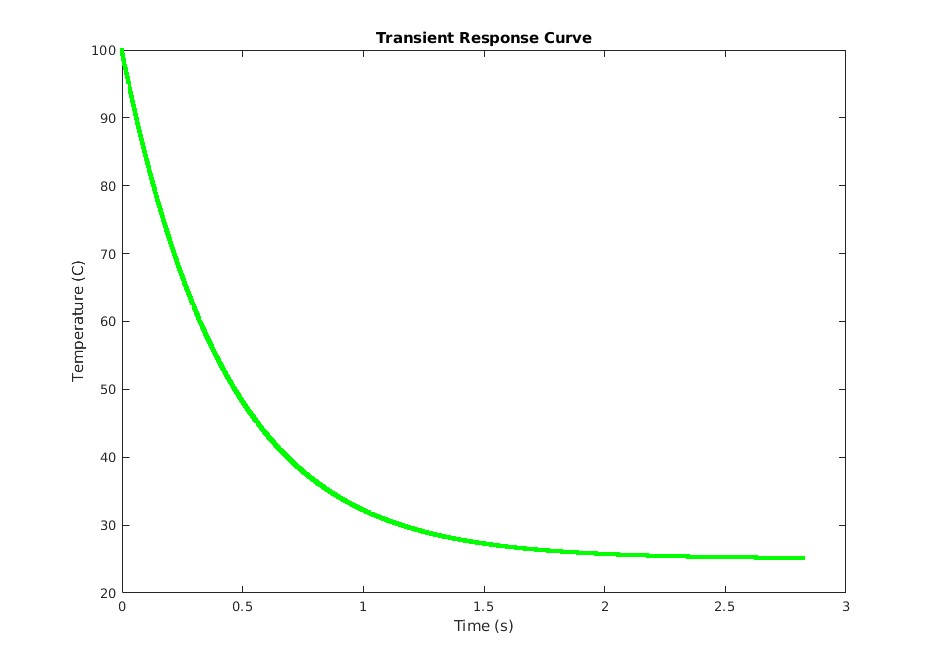
\includegraphics[width=.6\textwidth]{1TRC.jpg}
  \caption{Transient Response Curve for Part 1}
  \label{fig:1}
\end{figure}

\section*{Material Combinations}

\subsection*{Response Time}

Though it is a bit difficult to see, the weld constituted by 43\% tin and 57\% lead has the fastest response time.

\begin{figure}[H]
  \centering
  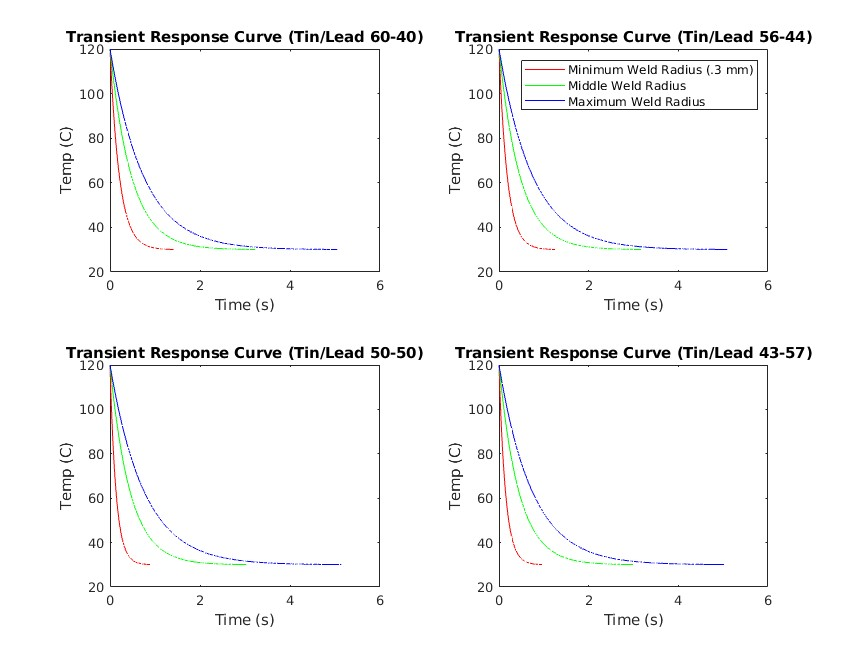
\includegraphics[width=.9\textwidth]{4TRC.jpg}
  \caption{The Transient Response Curves of the Four Tin/Lead Combinations for Minimum, Maximum, and Average Radius Values}
  \label{fig:2}
\end{figure}

\subsection*{Material Safety}

Given that a higher tin content increases the strength and reliability, in tandem with the fact that these will be used in engine safety monitoring systems, it would be best to use the weld with the highest tin content. As such, a weld with 60\% tin and 40\% lead would be the safest option.

\begin{figure}[H]
  \centering
  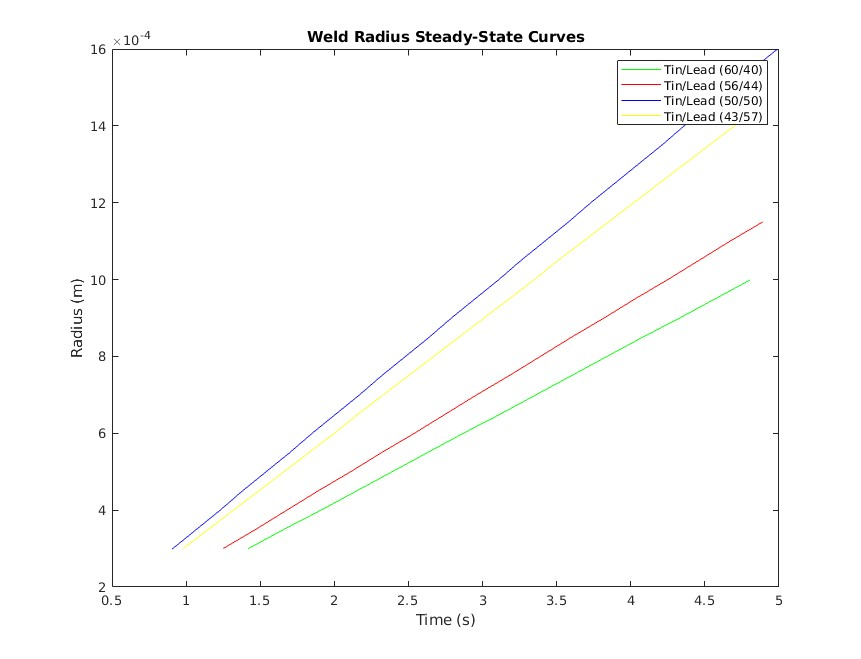
\includegraphics[width=.9\textwidth]{WeldRadius.jpg}
  \caption{The Maximum Weld Radii of Various Tin/Lead Combinations}
  \label{fig:3}
\end{figure}

\begin{algorithm}[H]
      \caption{CP3H1}\label{1}
      \begin{algorithmic}[1]
        \Procedure{Thermocouple Benchmark Tester}{}
        \State Ask user for inputs
        \Do 
            \State Add time step to time
            \State Calculate new sphere temperature using \textsc{rate\_of\_change()}
            \State Output values to file
        \doWhile{Sphere temperature minus liquid temperature is greater than .1$^{\circ}$C}
        \State Print steady-state time
    \Procedure{rate\_of\_change}{}
    \State Return $(3\cdot$ heat transfer coefficient $\cdot$ sphere and liquid temperature difference) $ / ($radius $\cdot$ density $\cdot$ specific heat)
      \end{algorithmic}
\end{algorithm}

\begin{algorithm}[H]
      \caption{CP3H2}\label{2}
      \begin{algorithmic}[1]
        \Procedure{Weld Radius Tester}{}
      \end{algorithmic}
      \begin{algorithmic}[1]
        \Procedure{user\_inputs}{}
          \State Ask user for global variable values
      \end{algorithmic}
      \begin{algorithmic}[1]
        \Procedure{rate\_of\_change}{}
          \State Return $(3\cdot$ heat transfer coefficient $\cdot$ sphere and liquid temperature difference) $ / ($radius $\cdot$ density $\cdot$ specific heat)
      \end{algorithmic}
      \begin{algorithmic}[1]
        \Procedure{gen\_time\_file}{}
          \State Use passed output object
          \State Use passed radius value
          \Do 
            \State Add time step to time
            \State Calculate new sphere temperature using \textsc{rate\_of\_change()}
            \State Output values to file
          \doWhile{Sphere temperature minus liquid temperature is greater than .1$^{\circ}$C}
      \end{algorithmic}
      \begin{algorithmic}[1]
        \Procedure{time\_to\_steady\_state}{}
          \State Use passed radius value
          \Do 
            \State Add time step to time
            \State Calculate new sphere temperature using \textsc{rate\_of\_change()}
          \doWhile{Sphere temperature minus liquid temperature is greater than .1$^{\circ}$C}
          \State Update time value
          \State Return time value
      \end{algorithmic}
      \begin{algorithmic}[1]
        \Procedure{gen\_rad\_file}{}
        \State Use passed output object
        \While{\textsc{time\_to\_steady\_state}(new radius value) is less than 5}
          \State Print \textsc{time\_to\_steady\_state}(new radius value) and new radius value to file
          \State Update radius value by radius step
      \end{algorithmic}
      \begin{algorithmic}[1]
        \Procedure{max\_weld\_size}{}
        \While{\textsc{time\_to\_steady\_state}(new radius value) is less than 5}
          \State Update radius value by radius step
        State Return radius value
      \end{algorithmic}
\end{algorithm}

\lstinputlisting[
    caption=CP3H1 Script, % Caption above the listing
	label=lst:L1, % Label for referencing this listing
	language=C++, % Use C++ functions/syntax highlighting
	frame=single, % Frame around the code listing
	showstringspaces=false, % Don't put marks in string spaces
	numbers=left, % Line numbers on left
	numberstyle=\tiny, % Line numbers styling
    backgroundcolor=\color{black!5}, % Set background color
    keywordstyle=\color{magenta!80}, % Set keyword color
    commentstyle=\color{blue!80}, % Set comment color
    stringstyle=\color{green!80}, % Set string color
    breaklines=true
  ]{CP3H1_MBROD.cpp}

\lstinputlisting[
    caption=CP3H2 Script, % Caption above the listing
	label=lst:L2, % Label for referencing this listing
	language=C++, % Use C++ functions/syntax highlighting
	frame=single, % Frame around the code listing
	showstringspaces=false, % Don't put marks in string spaces
	numbers=left, % Line numbers on left
	numberstyle=\tiny, % Line numbers styling
    backgroundcolor=\color{black!5}, % Set background color
    keywordstyle=\color{magenta!80}, % Set keyword color
    commentstyle=\color{blue!80}, % Set comment color
    stringstyle=\color{green!80}, % Set string color
    breaklines=true
  ]{CP3H2_MBROD.cpp}

%----------------------------------------------------------------------------------------

\end{document}
